The considerations of the previous Subsection lead to the reasonable
hypothesis that inter-sample distance is the key. Keeping training
sets uniform will result in smaller sets which still contain all
information required for training. Moreover, bad generalisation is
correlated to inter-set distance; therefore uniformisation can be as
well used to retain samples which are far away from the current
training set. We have then implemented an online version of the
uniformisation procedure, in order to test what would happen in a real
setting while the patient is freely moving around.

First of all, we reduced the sampling rate from $256$Hz to about
$25$Hz, since (see Section \ref{subsubsec:electrodes}) the bandwidth
of the EMG signal is limited in our experiment to about $10$Hz. This
got us a total training set of about $153000$ samples. The samples
were naturally chronologically ordered, so that they could be fed to
the system one by one as it would actually happen during continuous
acquisition of data from the patient's activity.

Furthermore, in an online setting no a-priori statistics about the
samples can be assumed. Therefore, as a measure of inter-sample
distance, we dropped the Mahalanobis distance (which requires a good
estimate of the covariance matrix) and resorted to Euclidean distance,
defined in the standard way. Normalisation was still used, as it is
essential for most machine learning methods, but the mean value and
standard deviation of the training sets were evaluated on-the-fly
without keeping the whole sets and re-evaluating them each
time. Testing samples were also normalised according to these
statistics.

We also tested the batch of samples for dimensionality reduction using
PCA, but found that no more than $2$ or $3$ dimensions could be
eliminated. Therefore we dropped the idea, also since PCA would
require, again, an estimate of the covariance matrix of the data set,
which is not available online.

The Online Uniformisation (OU) procedure, then, works like this: we
initially fix a minimum inter-sample distance $d$ and start
with an empty training set $S$. Then each time a new sample $\xx$ is
available, we check whether $dist(\xx,\xx_i)\leq d$, for at
least one $\xx_i \in S$: if this is the case, then $\xx$ is discarded;
otherwise, it is added to $S$.

The first question we were interested in was: does OU give us an
acceptable accuracy \emph{at all times}? That is: does $S$ constitute
a good training set, as the patient explores new regions of the input
space, and more and more samples are seen? In order to answer this
question we considered again the problem of SVM classification, and
let $S$ grow according to the OU procedure. Then, every about $1.5$
minutes of sampled data, that is every $2400$ samples, we trained the
SVM on $S$ and checked its accuracy on a testing set drawn from the
previously seen samples (but not in $S$, of course). This was done $5$
times with different splits of $S$, so to obtain a statistically
meaningful measure of accuracy. We chose to use a mid-range value of
$d = 0.21$ obtained from initial experiments, which would
result in a final training set of about $1800$ samples; moreover, we
used hyperparameters $C = 10^{1.5}$ and $\sigma = \sqrt{10}$, found by
grid search during the preliminary experiments. Figure \ref{fig:inc}
shows the results.

\begin{figure*}[!ht] \centering
  \begin{tabular}{cc}
    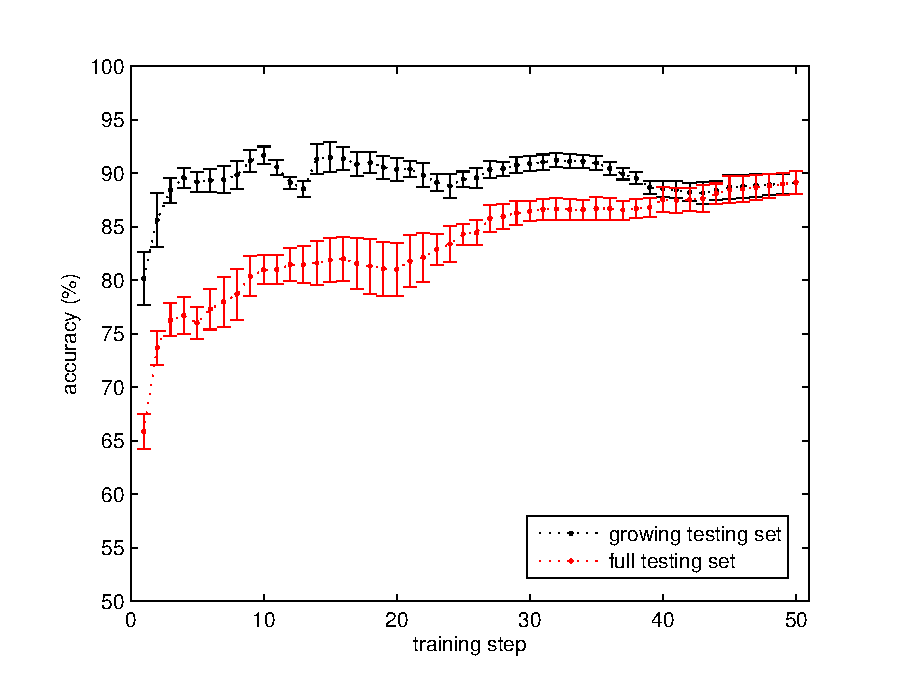
\includegraphics[width=0.45\textwidth]{figs/fig_resInc_OU21} &
    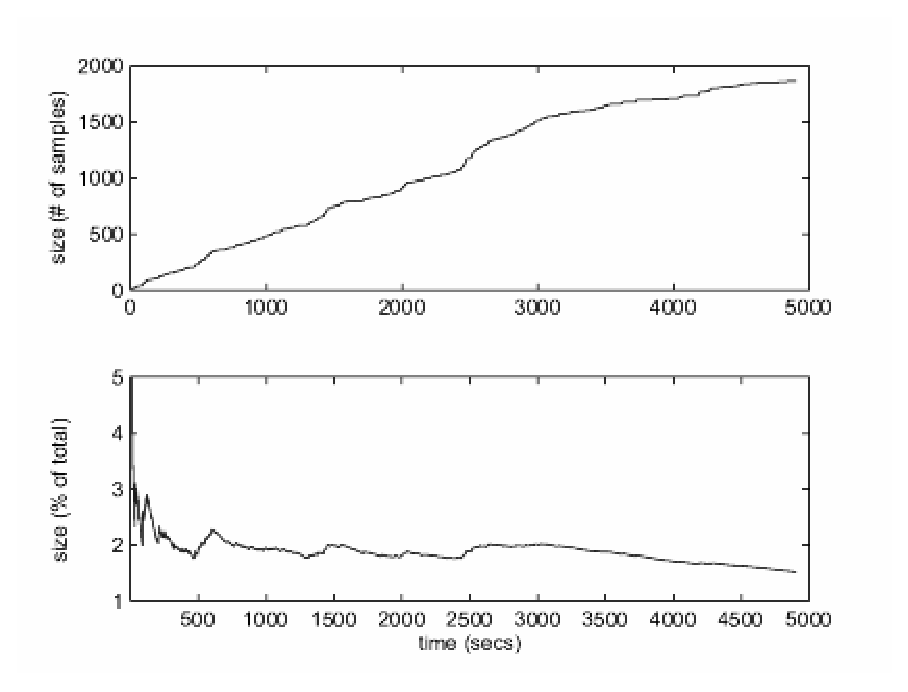
\includegraphics[width=0.45\textwidth]{figs/fig_growth_OU21} \\
    $(a)$ & $(b)$ \\
  \end{tabular}
  \caption{$(a)$: classification accuracy of an SVM, as the training set
    grows according to the OU procedure. \emph{Black curve:}
    growing testing set; \emph{Red curve:} full testing set. $(b)$:
    size of the online uniformised training set: number of samples
    (upper plot), fraction of the whole training set (lower plot).}
  \label{fig:inc}
\end{figure*}

Consider first the black curve in pane $(a)$ of the Figure: it is
apparent that, already after $4$ training steps, that is after some
$6$ minutes, the system can classify with an accuracy of about $90\%$,
as it was the case in the preliminary analysis (accuracy $89.57 \pm
0.94$). Notwithstanding some oscillations, the accuracy remains
substantially constant over the whole test and, at the end, is still
$89.14. \pm 1.05$. Consider now the red curve, representing the
accuracy obtained by the same models but on the \emph{whole} testing
set: now the system is being tested on samples drawn from zones of the
input space it has not yet seen; and, as one would expect, the
accuracy steadily increases, and it finally catches up with that
obtained by testing on the growing testing set.

Consider now pane $(b)$ of the Figure: the upper plot shows the size
of the online uniformised training set as the sample acquisition
proceeds; the lower plot shows the same curve as a fraction of the
full training set size. As time goes on, the OU procedure is letting
the uniform training set grow less and less; the fraction of the full
training set (lower plot) becomes smaller and smaller, being around
$1.5\%$ at the end.

From this we conclude that $(a)$ OU is keeping the training set
remarkably small in absolute terms, and smaller and smaller
percentage-wise, as more and more data is acquired; $(b)$ OU is
``letting in'' only relevant information, since the accuracy is
uniformly high if tested on a growing testing set, and ever growing if
tested upon a full testing set.

In other words, the OU procedure is effective in building a compact and
accurate training set for SVM classification.

What about the other approaches and problems? Figure \ref{fig:allres}
shows an all-inclusive set of results for all problems and approaches
considered, and for various values of the minimum distance threshold,
$d$, which was fixed at $0.21$ in the previous experiment.

\begin{figure*}[!ht] \centering
  \begin{tabular}{cc}
    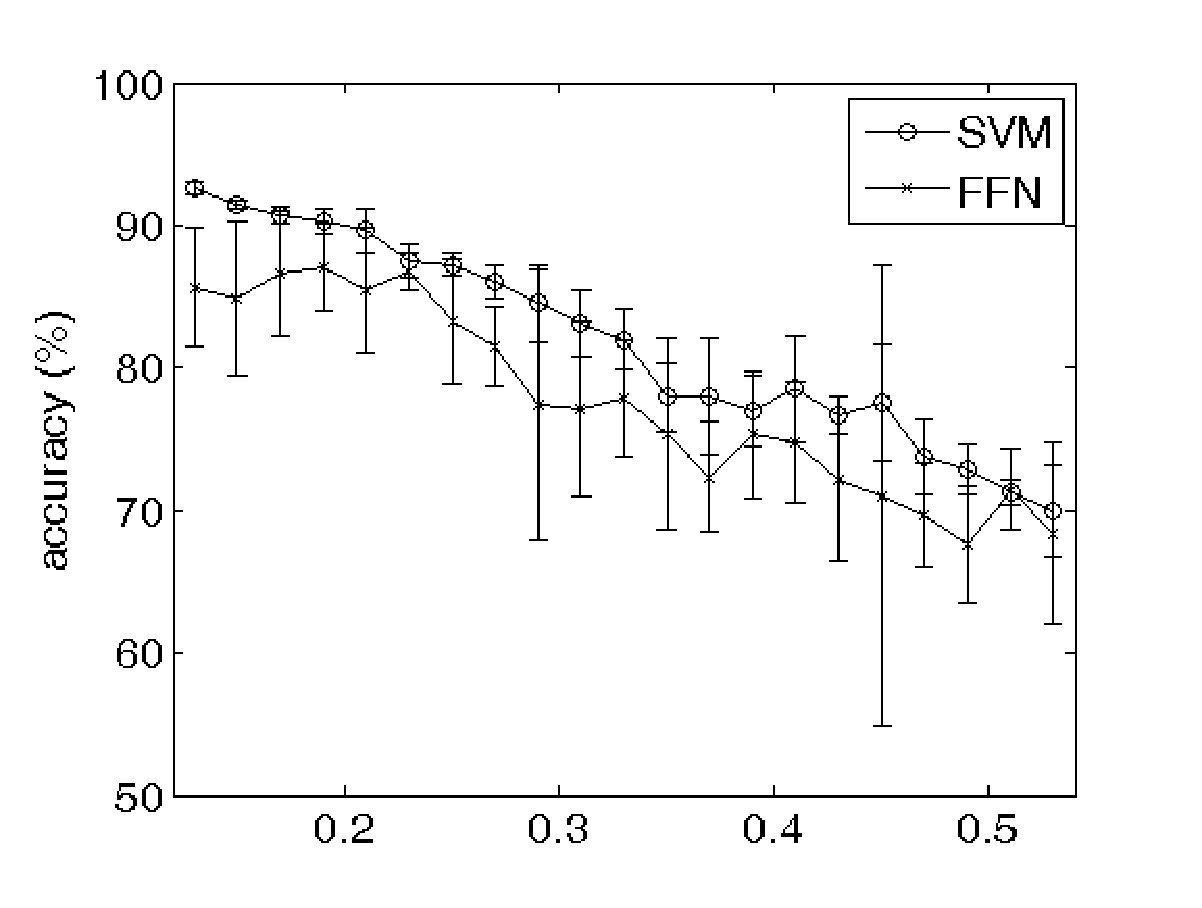
\includegraphics[width=0.45\textwidth]{figs/fig_all1} &
    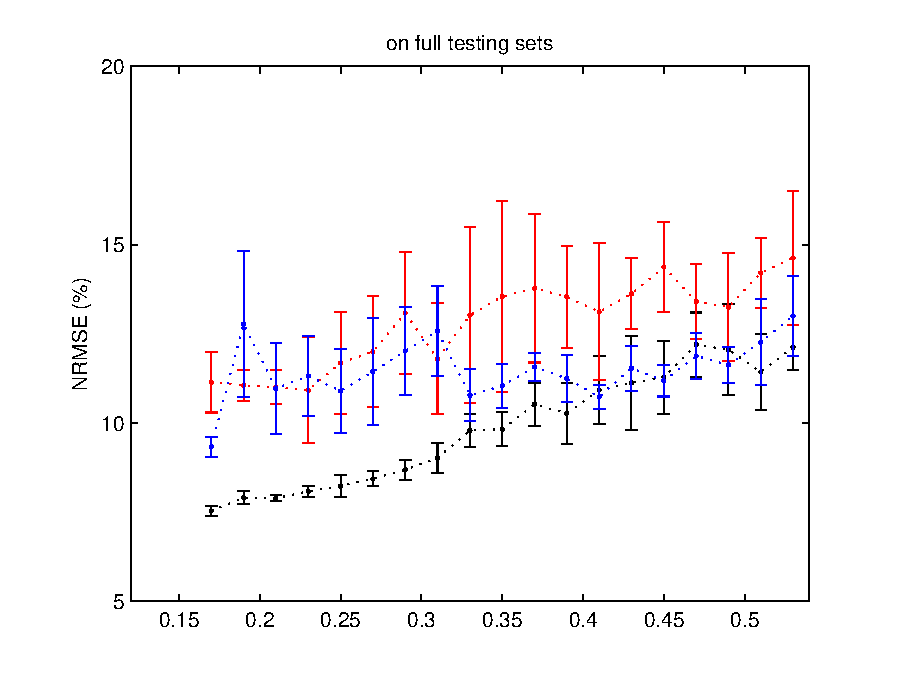
\includegraphics[width=0.45\textwidth]{figs/fig_all2} \\
    $(a)$ & $(b)$ \\
  \end{tabular}
  \caption{Classification and regression results using the OU
  procedure. $(a)$: classification, $(b)$: regression. Compare with
  Figure \ref{fig:TSsize} for the training set sizes.}
  \label{fig:allres}
\end{figure*}

As $d$ is increased from $0.13$ to $0.53$, all approaches show a
decreasing performance, as expected: in classification, the SVM is
almost uniformly better, going from $92.61\%$ for $d=0.13$ to
$70.01\%$ for $d=0.53$. The standard deviations for the SVM are, also,
uniformly smaller. In regression, again, the SVM is uniformly better
than the other approaches, ranging from $7.09\%$ NRMSE to $12.12\%$,
and it also shows uniformly smaller standard deviations. In both
problems, however, it must be remarked that the error bars largely
overlap, at least for $d>0.3$ in classification and $d>0.4$ for
regression.

One last consideration: as $d$ is increased, the size of the training
sets decreases like $d^{-10}$, since we are building a finite
partitioning of a subset of $\RR^{10}$ (see also Figure
\ref{fig:TSsize}, in which the training set size is plotted as a
function of $d$); whereas, it seems that the accuracy of all
approaches, and in both problems, only decreases linearly. This is a
remarkable feature of the OU procedure, since it will always be
possible to choose a polynomially smaller training set, for which we
can train a machine which will be only linearly worse.

\begin{figure}[!ht] \centering
  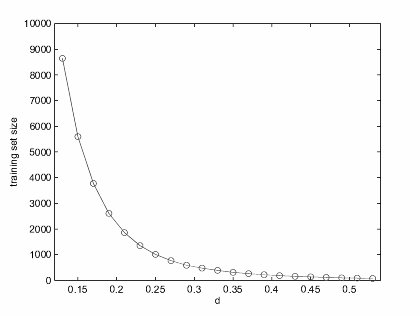
\includegraphics[width=0.45\textwidth]{figs/fig_allSize} \\
  \caption{Online uniformised training set size as $d$ changes.}
  \label{fig:TSsize}
\end{figure}

As a matter of fact, consider once again Figure \ref{fig:allres}, pane
$(b)$: at the far right end we have a SVM which has a still acceptable
error of $12.12\% \pm 0.64\%$, but whose training set, averaged over
the $5$ splits, consists of $77.4$ samples out of the original
$153000$!
